% ============================================================
%  Informe Técnico – Práctica 4: Clasificación de Objetos con Deep Learning
%  (fine tuning YOLO v26, detección y super resolución en GPU)
%  Visión por Computador – Universidad Politécnica Salesiana
%  Autores: Naspud Vivar Paul S. · Ramírez Saeteros Jennyfer C.
%  Período:  Marzo – Agosto 2026
% ============================================================
\documentclass[11pt,a4paper]{article}

\usepackage[utf8]{inputenc}
\usepackage[spanish,es-tabla]{babel}
\usepackage[margin=2.5cm]{geometry}
\usepackage{graphicx}
\usepackage{amsmath,amssymb}
\usepackage{booktabs}
\usepackage{multirow}
\usepackage{array}
\usepackage{subcaption}
\usepackage{float}
\usepackage{xcolor}
\usepackage{listings}
\usepackage{caption}
\usepackage{fancyhdr}
\usepackage{titlesec}
\usepackage[hidelinks,colorlinks=true,
            linkcolor=blue!55!black,
            citecolor=green!45!black,
            urlcolor=blue!65!black]{hyperref}

%% ── Listings ────────────────────────────────────────────────
\definecolor{bg}{rgb}{0.97,0.97,0.97}
\definecolor{kw}{rgb}{0.13,0.29,0.53}
\definecolor{cm}{rgb}{0.0,0.50,0.0}
\definecolor{st}{rgb}{0.58,0.0,0.82}
\definecolor{ln}{rgb}{0.5,0.5,0.5}

\lstdefinestyle{code}{
  backgroundcolor=\color{bg},
  basicstyle=\ttfamily\small,
  keywordstyle=\color{kw}\bfseries,
  commentstyle=\color{cm}\itshape,
  stringstyle=\color{st},
  numbers=none,
  breaklines=true,
  frame=none,
  xleftmargin=1em,
  showstringspaces=false,
  tabsize=2,
}

%% ── Línea decorativa para portada ──────────────────────────
\newcommand{\HRule}{\rule{\linewidth}{0.5mm}}

%% ── Encabezado/pie ──────────────────────────────────────────
\pagestyle{fancy}\fancyhf{}
\lhead{\small Visión por Computador -- UPS -- G9}
\rhead{\small Naspud \& Ramírez -- 2026}
\cfoot{\thepage}
\renewcommand{\headrulewidth}{0.4pt}

% ============================================================
\begin{document}
% ============================================================

%% ── PORTADA ─────────────────────────────────────────────────
%% ── PORTADA ─────────────────────────────────────────────────
\begin{titlepage}
\vbox{}\vbox{}
\begin{center}

% Logo UPS

\includegraphics[width=0.48\textwidth]{imagenes/logo-ups-home}\\[1cm]
\textsc{\LARGE Universidad Politécnica Salesiana}\\[0.4em]
\textsc{\large Ingeniería en Ciencias de la Computación}\\[1.2cm]

\textsc{\Large Materia: Visión por Computador}\\[0.5cm]
\vbox{}

% Título
\HRule\\[0.4cm]
{\LARGE\bfseries Clasificación de Objetos Usando Técnicas\\[0.25em]
de Deep Learning: fine tuning empleando\\[0.25em]
YOLO v26 y ejecución de redes de detección\\[0.25em]
de objetos y super resolución en unidades\\[0.25em]
gráficas de procesamiento (GPU)}\\[0.4cm]
\HRule\\[1.2cm]

% Autores y datos
\begin{minipage}[t]{0.45\textwidth}
  \begin{flushleft}\large
    \emph{Realizado por:}\\
    Naspud Vivar Paul Sebastian\\
    Ramírez Saeteros Jennyfer Camila
  \end{flushleft}
\end{minipage}
\hfill
\begin{minipage}[t]{0.45\textwidth}
  \begin{flushright}\large
    \emph{Docente:}\\
    Ing. Vladimir Robles Bykbaev\\[0.8em]
    \emph{Período:}\\
    Marzo -- Agosto 2026\\[0.8em]
    \emph{Grupo:} G9
  \end{flushright}
\end{minipage}

\vfill
{\large Informe Técnico -- Práctica 4}\\[0.3em]
{\small\today}

\end{center}
\end{titlepage}


%% ── ÍNDICES ─────────────────────────────────────────────────
\tableofcontents
\listoffigures
\listoftables
\newpage

%% ── SECCIONES ───────────────────────────────────────────────
% ============================================================
\section{Introducción}
% ============================================================

Las cargas de trabajo de visión por computador presentan una dicotomía
arquitectónica fundamental entre los dos procesadores disponibles en un equipo
moderno. La CPU es un procesador orientado a \emph{latencia}: pocos núcleos de
propósito general con frecuencias altas, jerarquías de caché profundas y lógica
compleja de predicción de saltos y ejecución fuera de orden, optimizados para
minimizar el tiempo de una tarea secuencial. La GPU, en cambio, es un procesador
orientado a \emph{throughput}: miles de núcleos simples agrupados en
multiprocesadores de flujo (SM) que ejecutan el mismo programa sobre miles de
datos simultáneamente bajo el modelo SIMT (\emph{Single Instruction, Multiple
Threads}) \cite{Owens2008}. La plataforma CUDA expone este paralelismo mediante
\emph{kernels} que se lanzan sobre mallas de bloques de hilos, con una memoria
de video dedicada (VRAM) de gran ancho de banda \cite{NVIDIA_CUDA}.

Esta ventaja no es gratuita: la GPU posee su propio espacio de memoria, por lo
que todo dato debe transferirse desde la RAM del sistema a la VRAM a través del
bus PCIe antes de ser procesado, y el resultado debe regresar por la misma vía.
Esta \emph{latencia de transferencia} es el costo fijo que decide si la
aceleración es rentable: en operaciones aritméticamente ligeras el viaje de ida
y vuelta puede consumir más tiempo que el propio cómputo, mientras que en redes
neuronales profundas ---donde las convoluciones se reducen a multiplicaciones
matriciales masivamente paralelas--- el cómputo domina y la GPU obtiene
aceleraciones de un orden de magnitud \cite{Paszke2019}. El consumo de VRAM,
además, limita el tamaño de lote y de modelo que la GPU puede alojar, del mismo
modo que la RAM limita a la CPU.

El presente informe cuantifica esta disyuntiva mediante un benchmark de tres
casos representativos de la práctica profesional en visión por computador:
\textbf{(A)} el ajuste fino (\emph{fine-tuning}) de la red de segmentación
YOLO26n sobre un conjunto de datos propio, comparando entrenamiento e
inferencia en CPU y GPU; \textbf{(B)} la inferencia en video con dos
generaciones de la familia YOLO (YOLOv12n y YOLO26n) y con la red de
superresolución Real-ESRGAN \cite{Wang2021}, midiendo cuadros por segundo (FPS)
y consumo de recursos en ambos dispositivos; y \textbf{(C)} un pipeline nativo
de detección de bordes en C++ con OpenCV, implementado en dos programas
equivalentes que ejecutan las mismas operaciones sobre \texttt{cv::Mat} (CPU) y
sobre \texttt{cv::cuda::GpuMat} (GPU) \cite{OpenCV_CUDA}.

\subsection*{Objetivos}
\begin{itemize}
  \item Comparar cuantitativamente el rendimiento de CPU y GPU en
        entrenamiento de redes profundas, inferencia de detección/segmentación
        y procesamiento clásico de imágenes.
  \item Registrar el estado del hardware durante cada prueba
        (\texttt{nvidia-smi}, \texttt{btop}, \texttt{top}, \texttt{lscpu}),
        incluyendo uso de CPU, RAM, VRAM, potencia y temperatura.
  \item Calcular la aceleración (\emph{speedup}) GPU/CPU de cada caso y
        justificar técnicamente por qué difiere entre ellos.
  \item Emitir recomendaciones de uso de hardware según el tipo de carga.
\end{itemize}

% ============================================================
\section{Desarrollo y Metodología}
% ============================================================

\subsection{Entorno Experimental}

Los experimentos se ejecutaron en dos entornos de hardware complementarios: el
entrenamiento del caso A se realizó en Google Colab (GPU Tesla T4), mientras
que los casos B y C se ejecutaron en una estación del laboratorio de Cómputo~8
(espacio de trabajo \texttt{\char`\~/paul} en el equipo
\texttt{cisco-optiplex7000}). La Tabla~\ref{tab:hardware} resume ambas
plataformas según lo reportado por \texttt{lscpu}, \texttt{free -h} y
\texttt{nvidia-smi}.

\begin{table}[H]
\centering
\caption{Entornos de hardware utilizados en el benchmark.}
\label{tab:hardware}
\setlength{\tabcolsep}{6pt}
\begin{tabular}{lcc}
  \toprule
  \textbf{Componente} & \textbf{Google Colab (Caso A)} & \textbf{Laboratorio (Casos B y C)} \\
  \midrule
  CPU              & Intel Xeon @ 2.20\,GHz (2 vCPU) & Intel Core i9-12900K (24 hilos) \\
  RAM              & 12.7\,GiB                        & 31\,GiB \\
  GPU              & NVIDIA Tesla T4                  & NVIDIA GeForce RTX 3070 \\
  VRAM             & 15\,360\,MiB                     & 8\,192\,MiB \\
  Driver / CUDA    & 580.82.07 / CUDA 13.0            & 535.274.02 / CUDA 12.2 \\
  Framework        & PyTorch 2.11.0+cu128             & PyTorch + OpenCV (WITH\_CUDA=ON) \\
  \bottomrule
\end{tabular}
\end{table}

La estación del laboratorio queda identificada de forma unívoca por su interfaz
de red \texttt{enp0s31f6}, con dirección MAC \texttt{08:92:04:e5:9d:24} y
dirección IP \texttt{172.16.12.194}, según la salida de \texttt{ip link}
mostrada en la Figura~\ref{fig:mac}.

\begin{figure}[H]
  \centering
  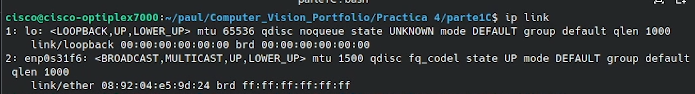
\includegraphics[width=0.95\textwidth]{imagenes/direccion_mac.png}
  \caption{Identificación de la estación de laboratorio mediante \texttt{ip link}:
           interfaz \texttt{enp0s31f6}, MAC \texttt{08:92:04:e5:9d:24}, dentro del
           espacio de trabajo \texttt{\char`\~/paul}.}
  \label{fig:mac}
\end{figure}

La metodología de medición fue uniforme en los tres casos: (i) cada
configuración CPU/GPU se ejecuta como proceso independiente para no contaminar
las mediciones; (ii) el tiempo por cuadro se mide con relojes monotónicos
(\texttt{std::chrono} en C++, \texttt{time.perf\_counter} en Python) y, cuando
interviene CUDA, se sincroniza el dispositivo antes y después de cronometrar
(\texttt{torch.cuda.synchronize()}) para no medir lanzamientos asíncronos;
(iii) el estado del sistema se monitorea en paralelo con \texttt{btop},
\texttt{top}, \texttt{ps} y \texttt{nvidia-smi}.

% ------------------------------------------------------------
\subsection{Caso A: Fine-Tuning de YOLO26n-seg}
\label{sec:casoA}

Se realizó el ajuste fino del modelo preentrenado \texttt{yolo26n-seg.pt}
(Ultralytics \cite{Ultralytics}) sobre el conjunto de datos propio
\textit{Tools segmentation}, etiquetado y exportado desde
Roboflow\footnote{\url{https://app.roboflow.com/paul-space-qcfcl/tools-segmentation-f2nhg-tf2cd/1}}:
3\,097 imágenes de herramientas (martillo, alicate,
tornillo, llave) divididas en 2\,709 de entrenamiento y 388 de prueba; la
validación se realizó sobre 406 imágenes con 772 instancias. El entrenamiento
se configuró con 60 épocas, resolución de entrada de $640\times640$, lote de 16
y paciencia de 15 épocas.

La sesión de Colab confirmó la disponibilidad del dispositivo CUDA antes de
entrenar: la Figura~\ref{fig:cuda_colab} muestra PyTorch 2.11.0+cu128 con
\texttt{CUDA disponible: True} y la Tesla T4 en reposo (3\,MiB de VRAM, 11\,W,
0\,\% de utilización) según \texttt{nvidia-smi}.

\begin{figure}[H]
  \centering
  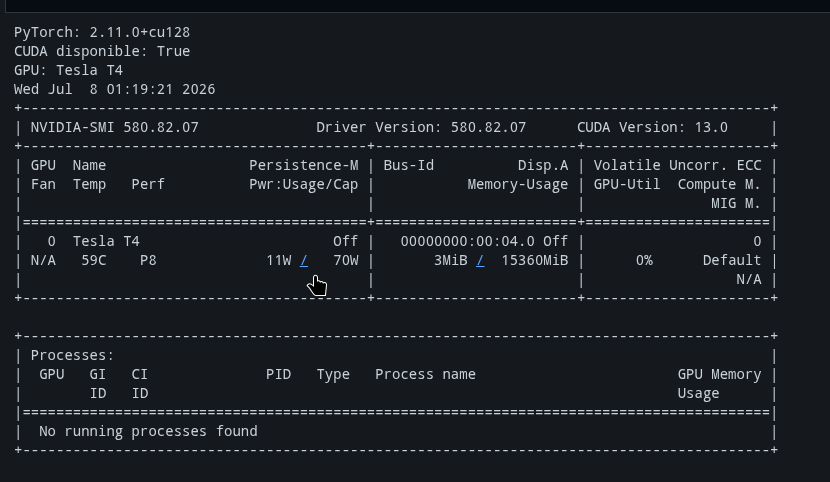
\includegraphics[width=0.85\textwidth]{imagenes/sectionA/cuda_disponible.png}
  \caption{Verificación del entorno en Google Colab: PyTorch 2.11.0+cu128,
           CUDA 13.0 y GPU Tesla T4 (15\,360\,MiB de VRAM) en estado de reposo.}
  \label{fig:cuda_colab}
\end{figure}

Del registro de entrenamiento se extraen la primera y la última época, que
evidencian la evolución del aprendizaje:

\begin{lstlisting}[style=code]
Epoch  GPU_mem  box_loss  seg_loss  cls_loss  dfl_loss   Instances  Size
 1/60    3.31G    0.8241     1.925     4.503  0.009851         67   640
        all  406  772  Box(P 0.539  R 0.189  mAP50 0.192  mAP50-95 0.137)
                       Mask(P 0.507  R 0.161  mAP50 0.151  mAP50-95 0.069)

60/60     4.6G    0.5509    0.7458    0.4008  0.009804         20   640
        all  406  772  Box(P 0.897  R 0.691  mAP50 0.792  mAP50-95 0.695)
                       Mask(P 0.898  R 0.692  mAP50 0.792  mAP50-95 0.606)
\end{lstlisting}

Entre la época 1 y la 60 la pérdida de clasificación cae de 4.503 a 0.4008
(un orden de magnitud) y la de segmentación de 1.925 a 0.7458, mientras el
mAP50 de cajas sube de 0.192 a 0.792. El consumo de VRAM se mantuvo estable
entre 3.31 y 4.6\,GiB de los 15\,GiB disponibles en la T4. Cada época tomó en
promedio 1\,min\,30\,s (144 lotes a 1.6--2.6\,it/s más la validación), lo que
arroja un total aproximado de \textbf{90 minutos de entrenamiento en GPU}. El
mismo entrenamiento lanzado sobre la CPU del entorno Colab (Xeon de 2 vCPU)
tomó entre 3.5 y 4 horas, con el kernel de Python saturando el procesador de
forma sostenida: \texttt{top} y \texttt{ps aux --sort=-\%cpu} registraron al
proceso \texttt{python3} en 87--100\,\% de CPU y hasta 5.2\,GiB de RAM
residente (41\,\% de la memoria del entorno), como se aprecia en el siguiente
extracto de monitoreo:

\begin{lstlisting}[style=code]
top - 17:12:08  load average: 1.33, 1.25, 0.82
%Cpu(s): 34.6 us, 18.6 sy, 45.8 id
MiB Mem : 12975.5 total, 3081.2 free, 6269.7 used

  PID USER  PR NI    VIRT    RES   SHR S  %CPU %MEM  COMMAND
 1931 root  20  0 7137180   5.2g 169120 R 100.0 41.2 python3 -m colab_kernel_lau
\end{lstlisting}

Las métricas finales de validación del modelo ajustado fueron
mAP50 $= 0.791$ y mAP50-95 $= 0.693$ para cajas, y mAP50 $= 0.790$ con
mAP50-95 $= 0.604$ para máscaras.

Posteriormente, los pesos entrenados se descargaron y se evaluaron en
inferencia local sobre CPU: predicción de imágenes estáticas del conjunto de
demostración y clasificación en vivo desde la cámara web, alcanzando alrededor
de \textbf{10.9 FPS} en tiempo real (Sección~\ref{sec:res_a}).

% ------------------------------------------------------------
\subsection{Caso B: Inferencia YOLOv12n vs.\ YOLO26n y Real-ESRGAN}
\label{sec:casoB}

El segundo caso compara, sobre la estación del laboratorio (i9-12900K +
RTX 3070), el rendimiento de inferencia de dos variantes ligeras de la familia
YOLO ---\texttt{yolo12n.pt} y \texttt{yolo26n.pt}--- ejecutadas sobre el mismo
video de prueba (\texttt{personas.mp4}) en cuatro combinaciones:
$\{$YOLOv12n, YOLO26n$\} \times \{$\texttt{cpu}, \texttt{cuda}$\}$. Cada
corrida superpone en pantalla el FPS instantáneo mientras \texttt{btop}
registra el estado de los 24 hilos de la CPU, la RAM y la GPU.

Como carga complementaria de cómputo intensivo se evaluó la red de
superresolución \textbf{Real-ESRGAN x4plus} (RRDBNet de 23 bloques residuales)
\cite{Wang2021} sobre un video en dos modalidades: procesamiento continuo de un
recorte central de $160\times160$\,px (ampliado $\times4$), y muestreo de un
cuadro completo cada 2 segundos. En la primera modalidad se registró el FPS en
vivo; en la segunda, el tiempo de procesamiento por cuadro: 1.12\,s en GPU
frente a 4.40\,s en CPU.

% ------------------------------------------------------------
\subsection{Caso C: Detección de Bordes en C++ (OpenCV / CUDA)}
\label{sec:casoC}

El tercer caso implementa en C++ un pipeline clásico de preprocesamiento sobre
video: conversión a escala de grises $\to$ suavizado gaussiano ($5\times5$,
$\sigma=1.5$) $\to$ erosión $\to$ dilatación $\to$ detección de bordes de Canny
(umbrales 50/150) \cite{Canny1986} en paralelo con ecualización de histograma.
Se compilaron \textbf{dos ejecutables independientes} a partir de dos archivos
fuente principales:

\begin{itemize}
  \item \texttt{src/pipeline\_cpu.cpp} $\to$ \texttt{preprocesamiento\_cpu}:
        toda la cadena sobre \texttt{cv::Mat}; compila con cualquier OpenCV.
  \item \texttt{src/pipeline\_gpu.cpp} $\to$ \texttt{preprocesamiento\_gpu}:
        la misma cadena sobre \texttt{cv::cuda::GpuMat}, con \emph{una única
        subida} (\texttt{upload}) del cuadro a VRAM y \emph{una única bajada}
        (\texttt{download}) del resultado, manteniendo todos los pasos
        intermedios en memoria de video. Requiere OpenCV compilado con
        \texttt{WITH\_CUDA=ON}, disponible como instalación de sistema en el
        laboratorio.
\end{itemize}

Separar ambas mediciones en programas distintos evita mezclar contadores de
tiempo en un mismo bucle. Cada ejecutable calcula un promedio móvil de 60
cuadros del tiempo de procesamiento y lo superpone en pantalla junto al FPS
equivalente; los filtros CUDA (gaussiano, morfológicos y Canny) se crean una
sola vez fuera del bucle para no recompilar el kernel en cada cuadro. Durante
la ejecución, el sistema se monitoreó con \texttt{btop} y \texttt{nvidia-smi}
(Sección~\ref{sec:res_c}).

% ============================================================
\section{Implementación}
% ============================================================

\subsection{Caso A: Dependencias, Selección de Dispositivo y Entrenamiento}

La instalación de dependencias en el entorno Python se reduce a dos paquetes
(Roboflow para descargar el dataset y Ultralytics para el modelo):

\begin{lstlisting}[style=code, language=bash]
pip install -q -U roboflow ultralytics
\end{lstlisting}

La selección explícita del dispositivo de cómputo se realiza consultando a
PyTorch; el mismo cuaderno corre en GPU o CPU sin cambios adicionales:

\begin{lstlisting}[style=code, language=Python]
import torch

print("PyTorch:", torch.__version__)
print("CUDA disponible:", torch.cuda.is_available())

device = 0 if torch.cuda.is_available() else "cpu"
\end{lstlisting}

El fine-tuning parte de los pesos preentrenados y apunta al \texttt{data.yaml}
exportado por Roboflow (rutas de \texttt{train/valid/test} y clases):

\begin{lstlisting}[style=code, language=Python]
from ultralytics import YOLO

model = YOLO("yolo26n-seg.pt")

train_results = model.train(
    data=str(YOLO_ROOT / "data.yaml"),
    epochs=60, imgsz=640, batch=16,
    device=device, patience=15,
    project="runs_practica4", name="yolo26n_seg_tools",
    pretrained=True,
)

metrics = model.val(data=str(YOLO_ROOT / "data.yaml"))
\end{lstlisting}

Para el benchmark de inferencia, toda medición sincroniza CUDA antes y después
del cronómetro; omitir esta sincronización subestimaría la latencia real, pues
los lanzamientos de kernels son asíncronos:

\begin{lstlisting}[style=code, language=Python]
def predict_timed(model, images, device, imgsz, half=False):
    if device == "cuda":
        torch.cuda.synchronize()
    t0 = time.perf_counter()
    model.predict(images, device=device, imgsz=imgsz,
                  half=half, verbose=False, conf=0.4)
    if device == "cuda":
        torch.cuda.synchronize()
    return (time.perf_counter() - t0) * 1000.0
\end{lstlisting}

\subsection{Caso B: Scripts de Inferencia en Video}

Cada combinación modelo/dispositivo se ejecuta cambiando dos constantes del
script \texttt{run\_yolo.py}; el FPS instantáneo se calcula por diferencia de
tiempos entre cuadros y se superpone al video anotado:

\begin{lstlisting}[style=code, language=Python]
MODEL_NAME = "yolo12n"   # "yolo12n" o "yolo26n"
DEVICE     = "cpu"       # "cuda" o "cpu"

model = YOLO(str(MODEL_PATH))
results = model.predict(frame, device=DEVICE, conf=0.4, verbose=False)

fps = 1.0 / max(now - prev_t, 1e-6)
\end{lstlisting}

Para Real-ESRGAN (\texttt{run\_superres.py}) el dispositivo se pasa
directamente a PyTorch; en GPU se activa media precisión (FP16) y se procesa
por mosaicos (\texttt{tile=128}) para no exceder la VRAM:

\begin{lstlisting}[style=code, language=Python]
model = RRDBNet(num_in_ch=3, num_out_ch=3, num_feat=64,
                num_block=23, num_grow_ch=32, scale=4)
upsampler = RealESRGANer(
    scale=4, model_path=str(MODEL_PATH), model=model,
    tile=128,
    half=(DEVICE == "cuda"),
    device=torch.device(DEVICE),
)
mejorado, _ = upsampler.enhance(crop, outscale=4)
\end{lstlisting}

\subsection{Caso C: Compilación y Vinculación de Librerías CUDA}

La infraestructura de compilación usa CMake orquestado por un Makefile. En el
laboratorio, OpenCV con CUDA (\texttt{WITH\_CUDA=ON} + \texttt{opencv\_contrib})
está \textbf{instalado a nivel de sistema}, por lo que
\texttt{find\_package(OpenCV)} lo localiza directamente y el objetivo GPU se
habilita de forma automática; los flags de inclusión y enlace contra las
librerías CUDA de OpenCV (\texttt{opencv\_cudaimgproc},
\texttt{opencv\_cudafilters}, \texttt{opencv\_cudaarithm}) los propaga CMake a
través de \texttt{\$\{OpenCV\_LIBS\}}:

\begin{lstlisting}[style=code]
cmake_minimum_required(VERSION 3.16)
project(Practica4Parte1C CXX)
set(CMAKE_CXX_STANDARD 17)

# Laboratorio: OpenCV con CUDA instalado en el sistema;
# find_package lo encuentra sin fijar OpenCV_DIR.
find_package(OpenCV REQUIRED)

add_executable(preprocesamiento_cpu src/pipeline_cpu.cpp)
target_link_libraries(preprocesamiento_cpu PRIVATE ${OpenCV_LIBS})
target_compile_options(preprocesamiento_cpu PRIVATE -O2 -Wall -Wextra)

if(OpenCV_CUDA_VERSION)   # solo si la build tiene WITH_CUDA=ON
    add_executable(preprocesamiento_gpu src/pipeline_gpu.cpp)
    target_link_libraries(preprocesamiento_gpu PRIVATE ${OpenCV_LIBS})
    target_compile_options(preprocesamiento_gpu PRIVATE -O2 -Wall -Wextra)
endif()
\end{lstlisting}

El Makefile expone los objetivos de compilación y ejecución:

\begin{lstlisting}[style=code]
all:
	cmake -B build -DCMAKE_BUILD_TYPE=Release -Wno-dev
	cmake --build build -j$(nproc)

run-cpu: all
	./build/preprocesamiento_cpu

run-gpu: all
	./build/preprocesamiento_gpu

clean:
	rm -rf build
\end{lstlisting}

\begin{lstlisting}[style=code, language=bash]
# Compilar y ejecutar en el laboratorio:
make            # configura y compila ambos ejecutables
make run-cpu    # pipeline sobre cv::Mat
make run-gpu    # pipeline sobre cv::cuda::GpuMat
\end{lstlisting}

El núcleo del programa GPU minimiza las transferencias PCIe: el cuadro sube una
sola vez a VRAM, las seis operaciones se encadenan sobre \texttt{GpuMat} y solo
el resultado final regresa a RAM:

\begin{lstlisting}[style=code, language=C++]
d_frame.upload(frame);                                   // CPU -> GPU (unica subida)
cv::cuda::cvtColor(d_frame, d_gris, cv::COLOR_BGR2GRAY);
gaussianFilter->apply(d_gris, d_suavizado);
erodeFilter->apply(d_suavizado, d_erosionado);
dilateFilter->apply(d_erosionado, d_dilatado);
cannyDetector->detect(d_dilatado, d_bordes);
cv::cuda::equalizeHist(d_dilatado, d_ecualizado);
d_resultado.download(resultado);                         // GPU -> CPU (unica bajada)
\end{lstlisting}

Antes de procesar, el programa valida la presencia de un dispositivo CUDA:

\begin{lstlisting}[style=code, language=C++]
if (cv::cuda::getCudaEnabledDeviceCount() == 0) {
    std::cerr << "No se detecto GPU CUDA-capable via OpenCV.\n";
    return 1;
}
cv::cuda::printShortCudaDeviceInfo(cv::cuda::getDevice());
\end{lstlisting}

% ============================================================
\section{Resultados y Discusión}
% ============================================================

\subsection{Caso A: Entrenamiento e Inferencia del Modelo Ajustado}
\label{sec:res_a}

La Tabla~\ref{tab:epochs} contrasta la primera y la última época del
entrenamiento en GPU. La caída simultánea de las tres pérdidas principales y el
incremento de mAP50 de cajas desde 0.192 hasta 0.792 confirman una convergencia
sana, sin señales de sobreajuste dentro de la paciencia configurada.

\begin{table}[H]
\centering
\caption{Evolución del entrenamiento de YOLO26n-seg (Tesla T4, 60 épocas).}
\label{tab:epochs}
\setlength{\tabcolsep}{6pt}
\begin{tabular}{lcc}
  \toprule
  \textbf{Métrica} & \textbf{Época 1/60} & \textbf{Época 60/60} \\
  \midrule
  VRAM ocupada (\texttt{GPU\_mem})    & 3.31\,GiB & 4.60\,GiB \\
  \texttt{box\_loss}                  & 0.8241    & 0.5509 \\
  \texttt{seg\_loss}                  & 1.9250    & 0.7458 \\
  \texttt{cls\_loss}                  & 4.5030    & 0.4008 \\
  Box: precisión / recall             & 0.539 / 0.189 & 0.897 / 0.691 \\
  Box: mAP50 / mAP50-95               & 0.192 / 0.137 & 0.792 / 0.695 \\
  Mask: mAP50 / mAP50-95              & 0.151 / 0.069 & 0.792 / 0.606 \\
  Tiempo de la época                  & 1\,min\,28\,s + 31\,s val. & 55.4\,s + 5.5\,s val. \\
  \bottomrule
\end{tabular}
\end{table}

En tiempo total, las 60 épocas en la Tesla T4 (a un promedio de
$\approx$1\,min\,30\,s por época) sumaron \textbf{$\approx$90 minutos},
frente a las \textbf{3.5--4 horas} que tomó el mismo entrenamiento sobre la CPU
Xeon de 2 vCPU del entorno, es decir, una aceleración de
\textbf{2.4--2.7$\times$} incluso contra una GPU de gama de inferencia como la
T4 y con un dataset que satura el pipeline de datos. Cabe señalar que durante
el entrenamiento en CPU el proceso Python se mantuvo clavado en 87--100\,\% de
uso de procesador, mientras que en GPU la CPU quedó libre para el pipeline de
carga de imágenes.

La matriz de confusión del modelo final (Figura~\ref{fig:confusion}) muestra
diagonales dominantes en las cuatro clases (332 aciertos en \textit{hammer},
177 en \textit{wrench}, 155 en \textit{screw}); el principal modo de error es
la confusión con el fondo (58, 42 y 27 instancias respectivamente), típico de
objetos delgados como tornillos y llaves.

\begin{figure}[H]
  \centering
  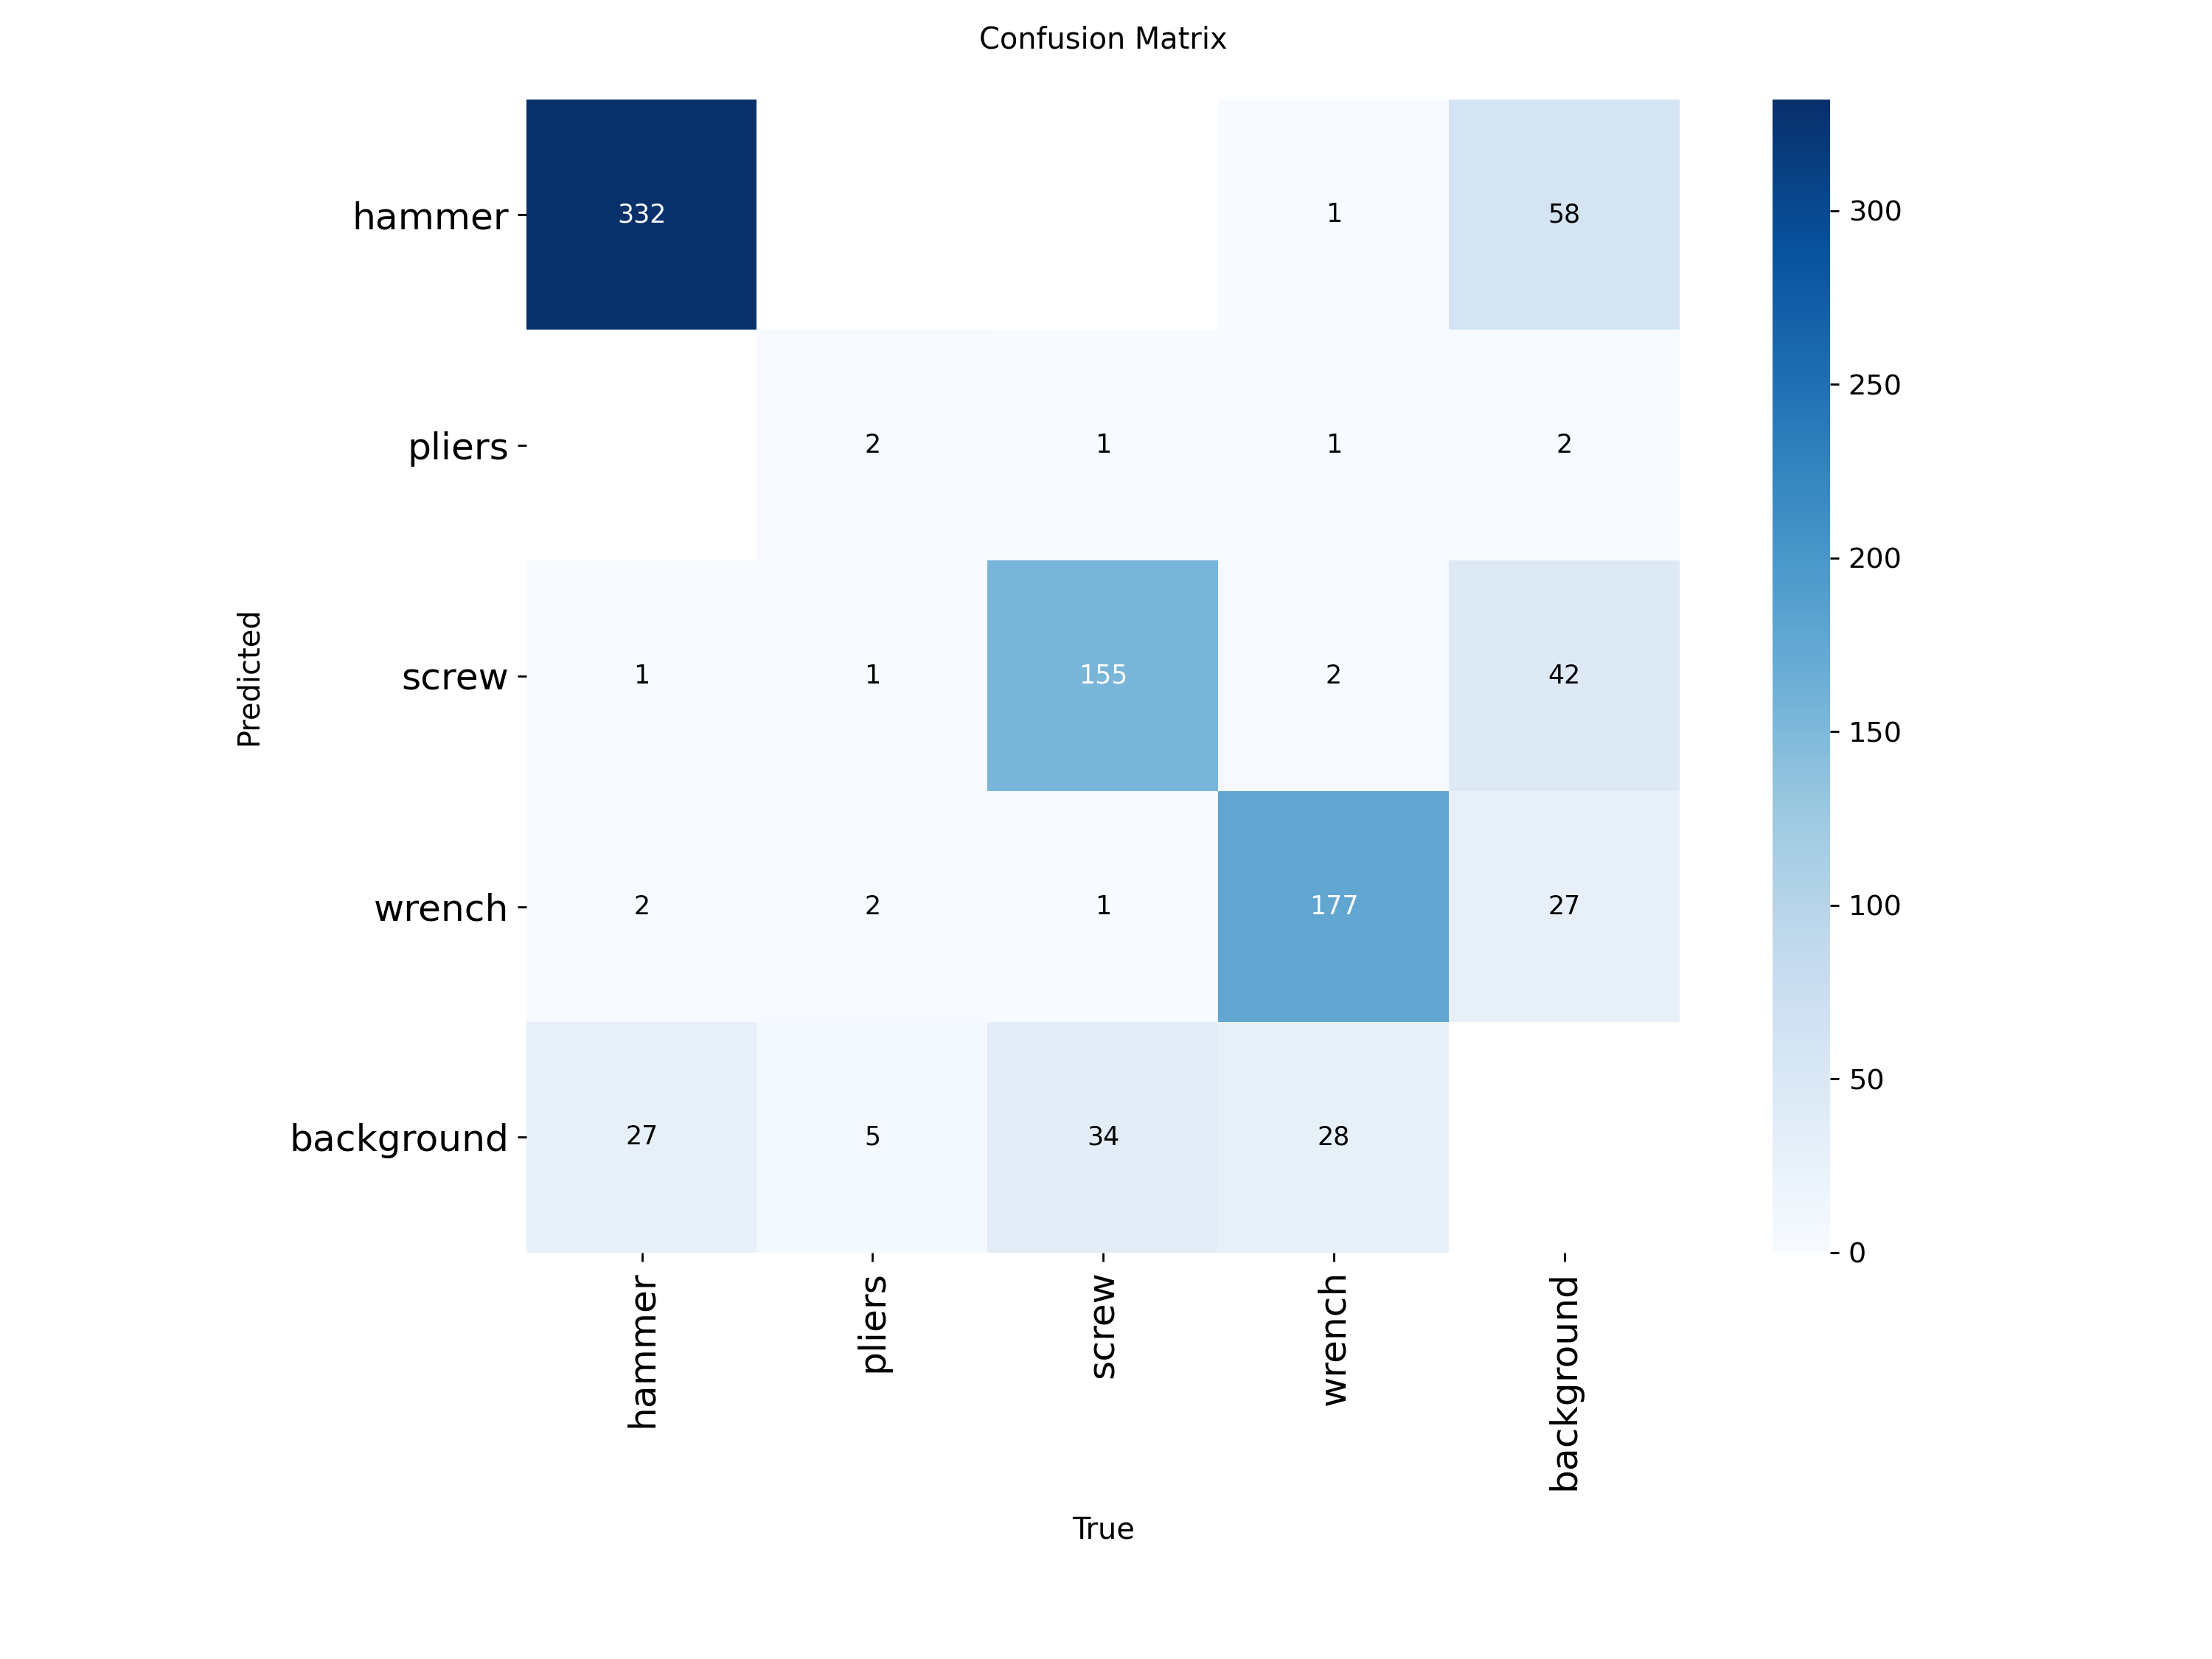
\includegraphics[width=0.8\textwidth]{imagenes/sectionA/matriz_confusion.png}
  \caption{Matriz de confusión del modelo YOLO26n-seg ajustado sobre el
           conjunto de validación (4 clases + fondo).}
  \label{fig:confusion}
\end{figure}

En la evaluación local (CPU del equipo de desarrollo) sobre el subconjunto de
test exportado, las métricas descienden (mAP50 $= 0.295$, precisión $= 0.619$,
recall $= 0.261$; Figura~\ref{fig:metricas_eval}), lo que se atribuye al cambio
de dominio de las imágenes locales respecto al conjunto de Roboflow. El tiempo
medio de predicción en CPU fue de \textbf{98.6\,ms por imagen}
(Figura~\ref{fig:tiempo_cpu}), equivalente a $\approx$10 FPS teóricos, cifra
coherente con los \textbf{10.9 FPS} medidos con la cámara web en vivo
(Figura~\ref{fig:inferencia_local}).

\begin{figure}[H]
  \centering
  \begin{subfigure}[b]{0.55\textwidth}
    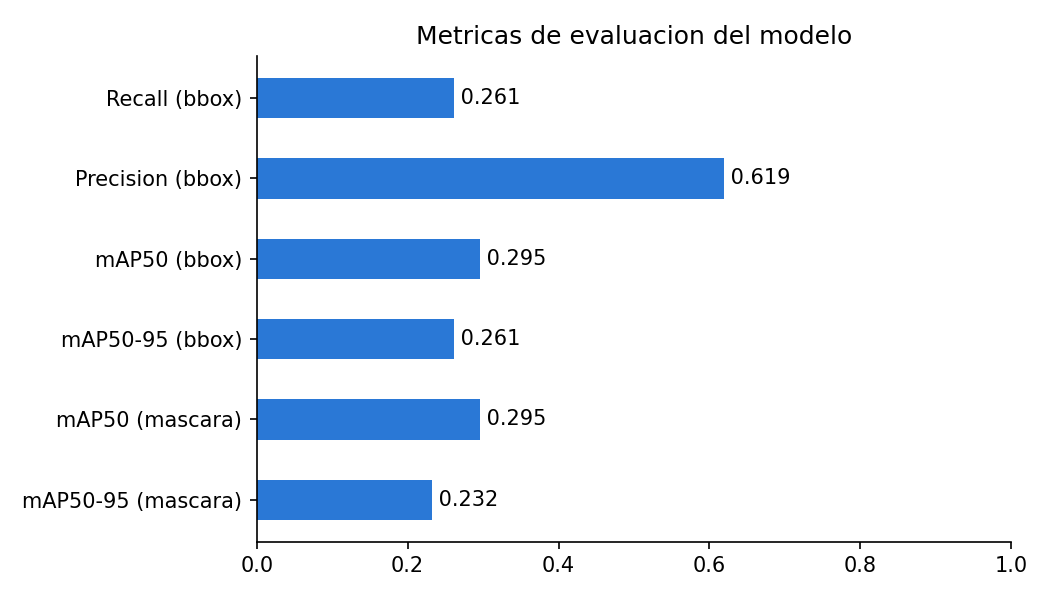
\includegraphics[width=\textwidth]{imagenes/sectionA/metricas_evaluacion.png}
    \caption{Métricas de la evaluación local.}
    \label{fig:metricas_eval}
  \end{subfigure}\hfill
  \begin{subfigure}[b]{0.42\textwidth}
    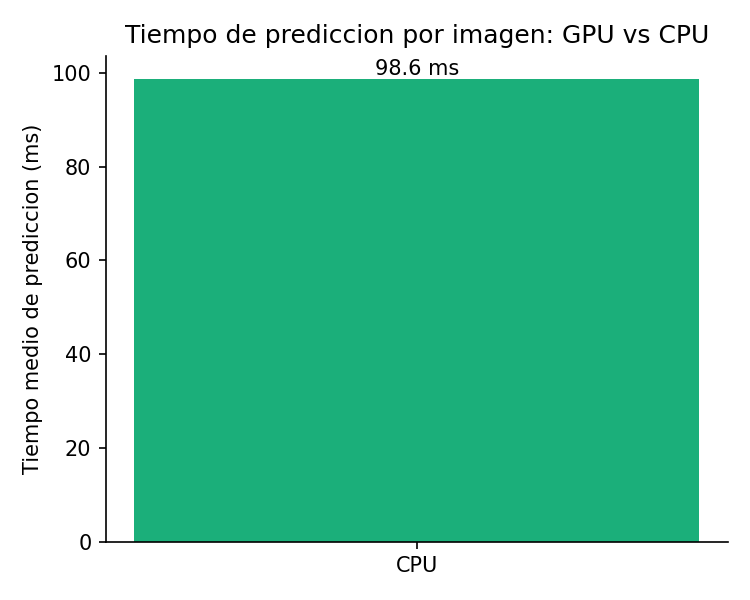
\includegraphics[width=\textwidth]{imagenes/sectionA/tiempo_prediccion_gpu_vs_cpu.png}
    \caption{Tiempo medio de predicción (CPU): 98.6\,ms.}
    \label{fig:tiempo_cpu}
  \end{subfigure}
  \caption{Evaluación del modelo ajustado en el equipo local (inferencia CPU).}
  \label{fig:eval_local}
\end{figure}

\begin{figure}[H]
  \centering
  \begin{subfigure}[b]{0.55\textwidth}
    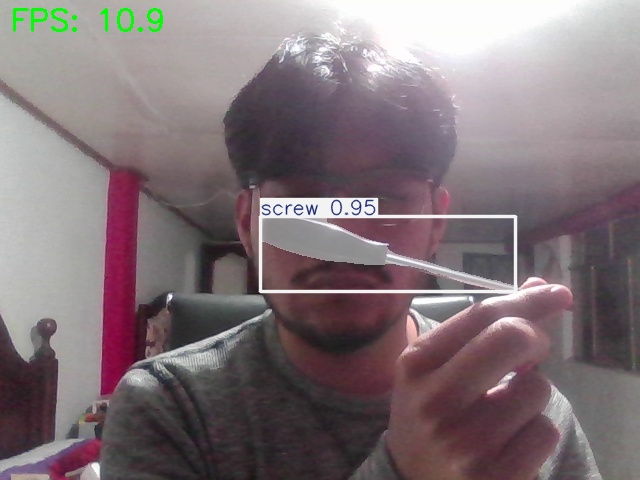
\includegraphics[width=\textwidth]{imagenes/sectionA/yolo_camara.jpg}
    \caption{Cámara web en vivo: \textit{screw} 0.95 a 10.9 FPS (CPU).}
  \end{subfigure}\hfill
  \begin{subfigure}[b]{0.42\textwidth}
    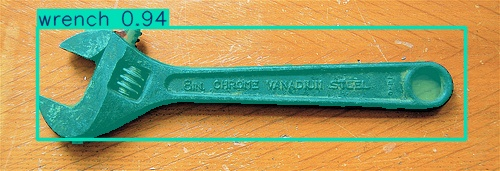
\includegraphics[width=\textwidth]{imagenes/sectionA/yolo_imagen.JPEG}
    \caption{Imagen estática: \textit{wrench} 0.94.}
  \end{subfigure}
  \caption{Inferencia local del modelo YOLO26n-seg ajustado.}
  \label{fig:inferencia_local}
\end{figure}

\subsection{Caso B: YOLOv12n vs.\ YOLO26n y Real-ESRGAN}
\label{sec:res_b}

La Figura~\ref{fig:yolo_fps} recoge las cuatro corridas sobre el mismo video en
la estación del laboratorio. Los FPS superpuestos en pantalla y el estado de
\texttt{btop} en cada captura resumen el comportamiento: en CPU, ambos modelos
reparten la carga entre los 24 hilos del i9-12900K (núcleos entre 27 y 84\,\%,
reloj a 4.9\,GHz, 67--70\,$^{\circ}$C) con la GPU ociosa (1\,\%, 436\,MiB de
base); en CUDA, la situación se invierte: la CPU cae a 6--7\,\% con el reloj
reducido a 0.8--1.3\,GHz y la VRAM sube a 743\,MiB.

\begin{figure}[H]
  \centering
  \begin{subfigure}[b]{0.49\textwidth}
    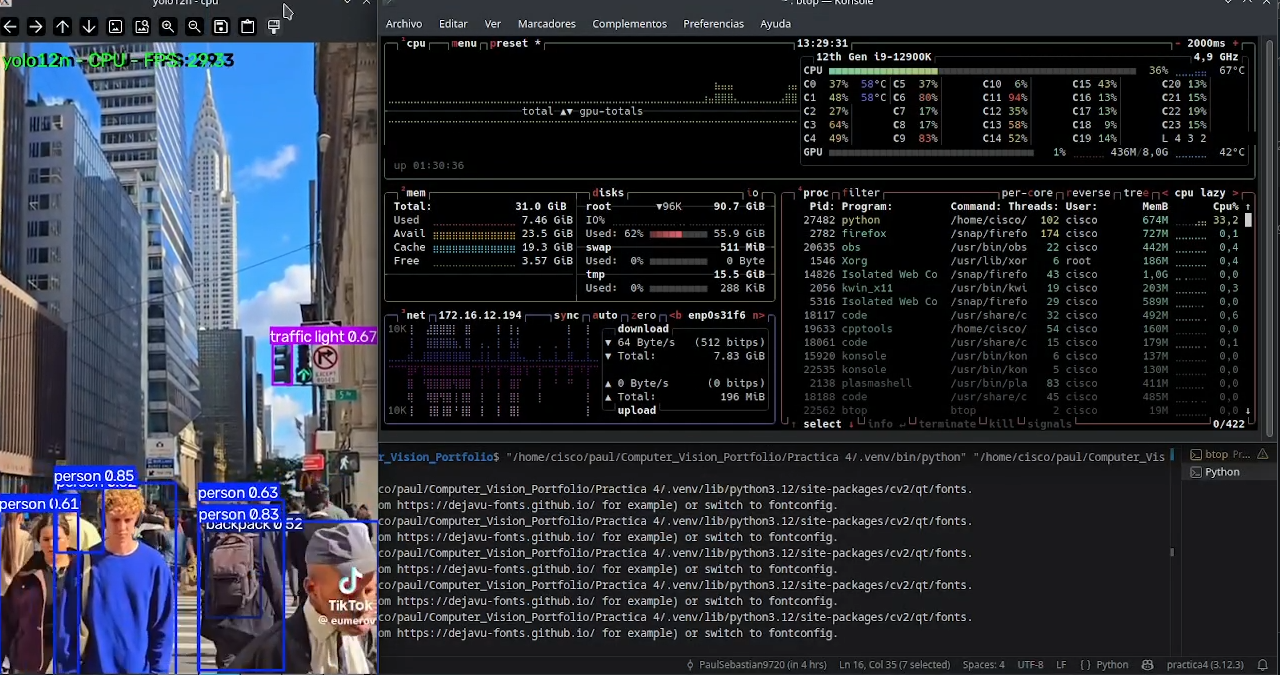
\includegraphics[width=\textwidth]{imagenes/sectionB/yolo/cpu_yolo12.png}
    \caption{YOLOv12n en CPU: 29.3 FPS.}
  \end{subfigure}\hfill
  \begin{subfigure}[b]{0.49\textwidth}
    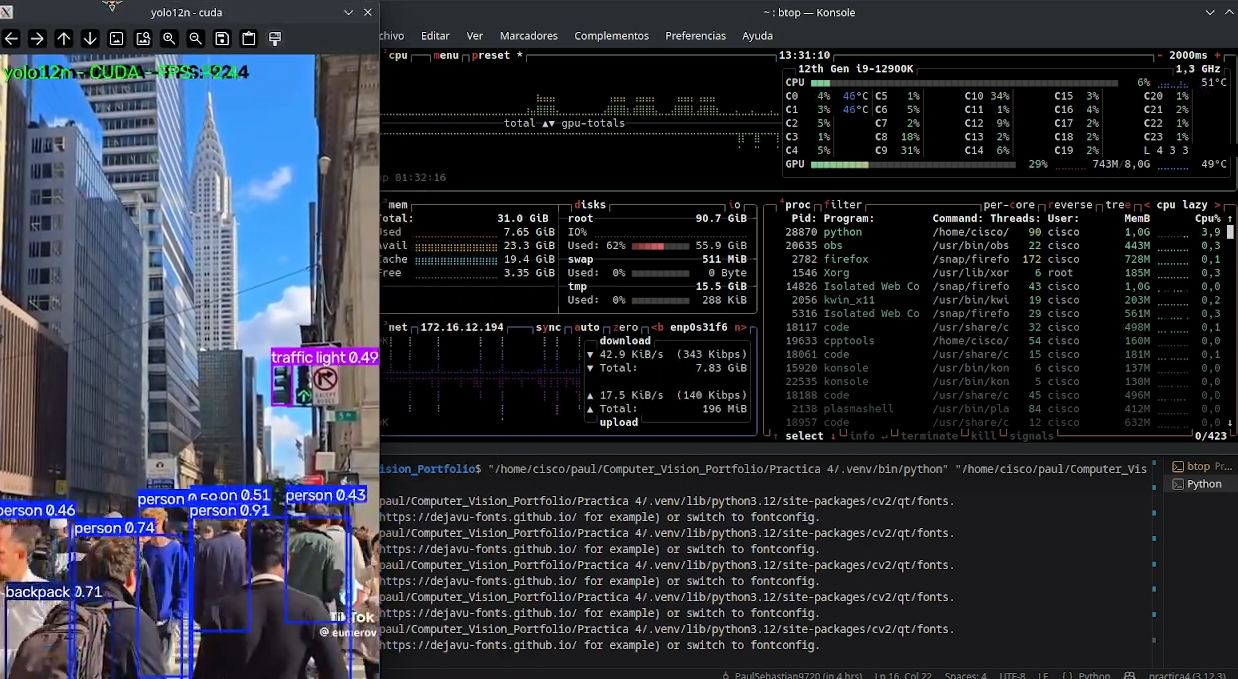
\includegraphics[width=\textwidth]{imagenes/sectionB/yolo/gpu_yolo12.png}
    \caption{YOLOv12n en CUDA: 122.4 FPS.}
  \end{subfigure}\\[0.6em]
  \begin{subfigure}[b]{0.49\textwidth}
    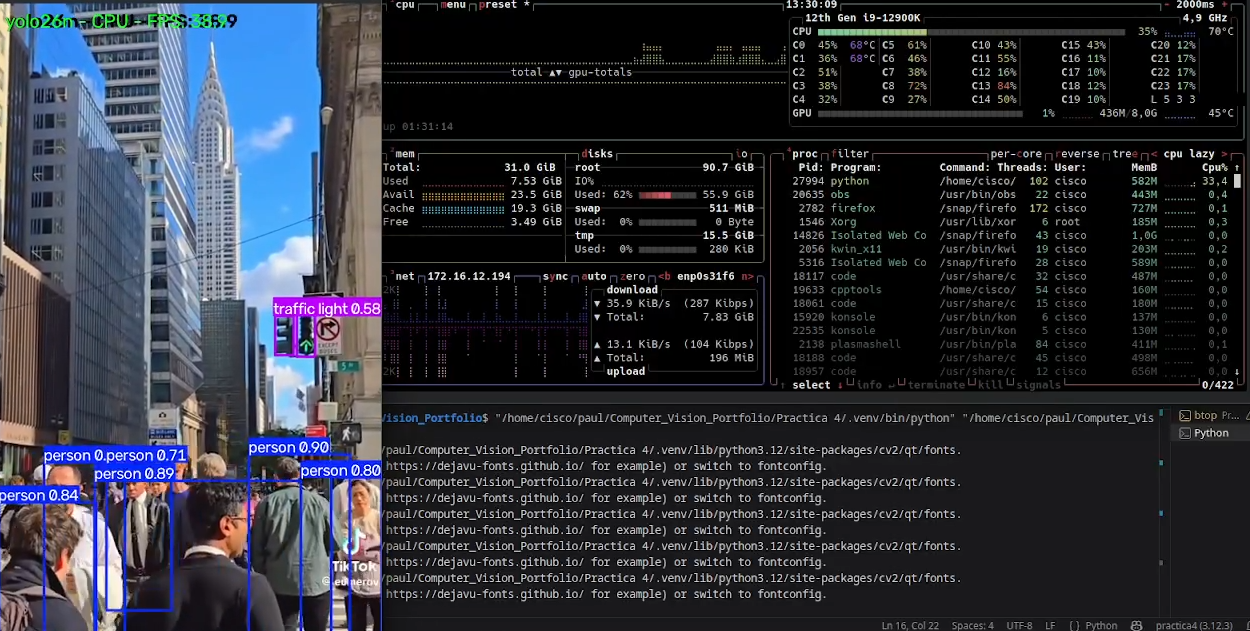
\includegraphics[width=\textwidth]{imagenes/sectionB/yolo/cpu_yolo26.png}
    \caption{YOLO26n en CPU: 38.9 FPS.}
  \end{subfigure}\hfill
  \begin{subfigure}[b]{0.49\textwidth}
    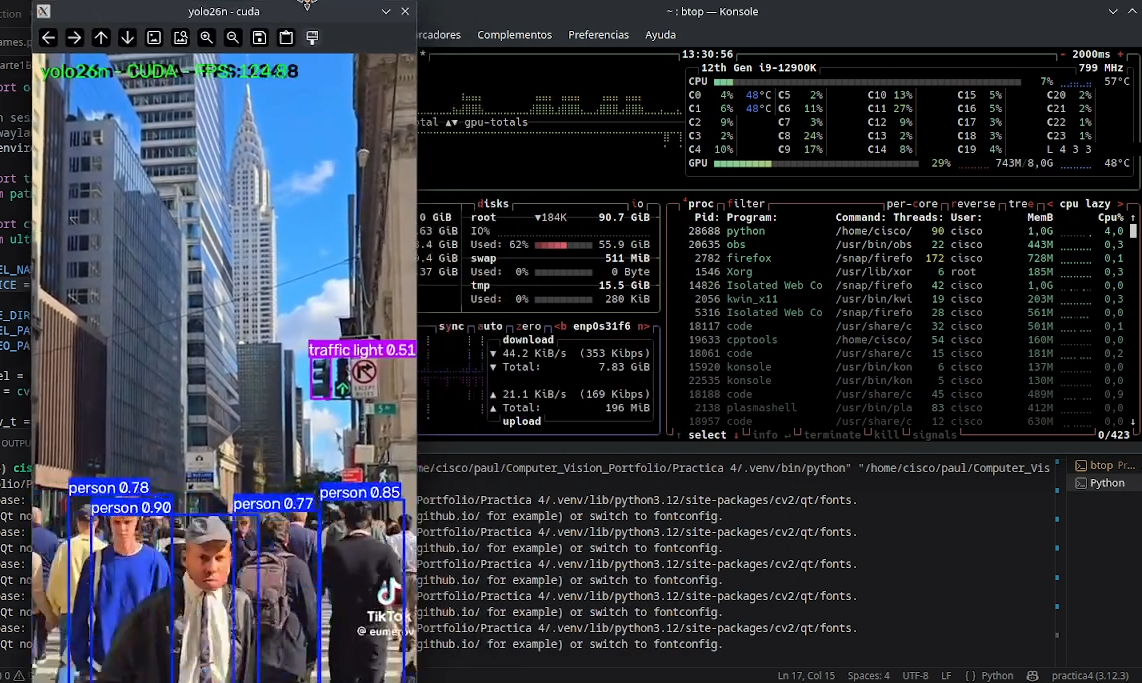
\includegraphics[width=\textwidth]{imagenes/sectionB/yolo/gpu_yolo26.png}
    \caption{YOLO26n en CUDA: 124.8 FPS.}
  \end{subfigure}
  \caption{Inferencia sobre video con dos variantes YOLO en la estación del
           laboratorio (i9-12900K / RTX 3070), con monitoreo \texttt{btop}
           simultáneo.}
  \label{fig:yolo_fps}
\end{figure}

\begin{table}[H]
\centering
\caption{FPS medidos por modelo y dispositivo (video \texttt{personas.mp4}).}
\label{tab:yolo_fps}
\begin{tabular}{lccc}
  \toprule
  \textbf{Modelo} & \textbf{CPU (FPS)} & \textbf{GPU (FPS)} & \textbf{Speedup} \\
  \midrule
  YOLOv12n & 29.3 & 122.4 & 4.2$\times$ \\
  YOLO26n  & 38.9 & 124.8 & 3.2$\times$ \\
  \bottomrule
\end{tabular}
\end{table}

Dos observaciones se desprenden de la Tabla~\ref{tab:yolo_fps}. Primera: en
CPU, YOLO26n supera a YOLOv12n (38.9 vs.\ 29.3 FPS), reflejo de las
optimizaciones de arquitectura de la generación más reciente. Segunda: en GPU
ambos modelos convergen a $\approx$122--125 FPS, señal de que la inferencia
deja de ser el cuello de botella y el límite pasa a estar en las etapas de CPU
del bucle (decodificación del video, anotación del cuadro y visualización). En
ese régimen, la GPU queda parcialmente ociosa esperando cuadros.

En Real-ESRGAN la brecha es cualitativamente mayor
(Figura~\ref{fig:esrgan_frames}): el recorte de $160\times160$ ampliado
$\times$4 corre a \textbf{0.36 FPS en CPU} frente a \textbf{1.57 FPS en CUDA};
en la modalidad de cuadro completo muestreado cada 2\,s, los tiempos fueron
4.40\,s (CPU) frente a 1.12\,s (GPU), un speedup de \textbf{3.9$\times$}. El
costo sistémico de la vía CPU es notable (Figura~\ref{fig:esrgan_btop}): 52\,\%
de uso agregado de los 24 hilos con picos de \textbf{91\,$^{\circ}$C} a
4.9\,GHz, mientras que en CUDA la GPU trabaja al 62\,\% con 899\,MiB de VRAM y
la CPU desciende a 5\,\% (44\,$^{\circ}$C).

\begin{figure}[H]
  \centering
  \begin{subfigure}[b]{0.49\textwidth}
    
\includegraphics[width=\textwidth]{imagenes/sectionB/mejora/cpu_frame_1.png}
    \caption{CPU: 0.36 FPS.}
  \end{subfigure}\hfill
  \begin{subfigure}[b]{0.49\textwidth}
    
\includegraphics[width=\textwidth]{imagenes/sectionB/mejora/gpu_frame_1.png}
    \caption{CUDA: 1.57 FPS.}
  \end{subfigure}
  \caption{Real-ESRGAN x4plus sobre recorte central (original interpolado
           vs.\ superresolución).}
  \label{fig:esrgan_frames}
\end{figure}

\begin{figure}[H]
  \centering
  \begin{subfigure}[b]{0.49\textwidth}
    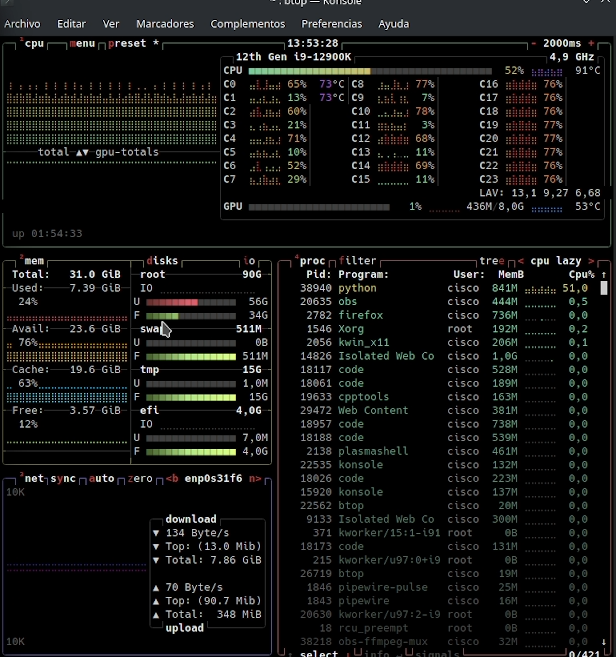
\includegraphics[width=\textwidth]{imagenes/sectionB/mejora/cpu_frame_1_btop.png}
    \caption{Modo CPU: 52\,\% agregado, 4.9\,GHz, 91\,$^{\circ}$C; GPU 1\,\%.}
  \end{subfigure}\hfill
  \begin{subfigure}[b]{0.49\textwidth}
    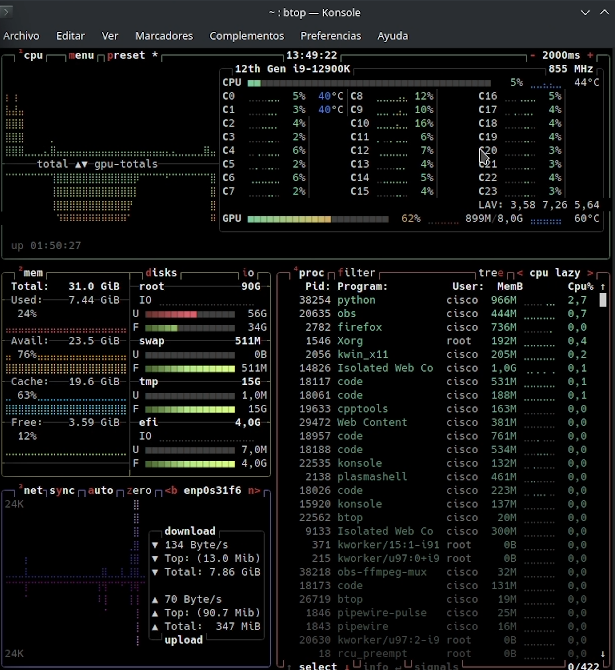
\includegraphics[width=\textwidth]{imagenes/sectionB/mejora/gpu_frame_1_btop.png}
    \caption{Modo CUDA: GPU 62\,\%, 899\,MiB VRAM; CPU 5\,\%.}
  \end{subfigure}
  \caption{Monitoreo \texttt{btop} durante Real-ESRGAN: la carga migra por
           completo de la CPU a la GPU.}
  \label{fig:esrgan_btop}
\end{figure}

\subsection{Caso C: Pipeline de Bordes en C++}
\label{sec:res_c}

Las Figuras~\ref{fig:bordes_cpu} y~\ref{fig:bordes_gpu} muestran ambos
ejecutables procesando video con el HUD de tiempo por cuadro: la versión CPU
promedia \textbf{6.666\,ms/cuadro (150 FPS)} y la versión GPU-only
\textbf{2.314\,ms/cuadro (432 FPS)}, es decir, un speedup de
\textbf{2.9$\times$}. Durante la corrida GPU, \texttt{nvidia-smi}
(Figura~\ref{fig:nvidia_smi_c}) reporta al proceso
\texttt{./build/preprocesamiento\_gpu} con apenas \textbf{172\,MiB de VRAM},
utilización del \textbf{2\,\%} y 47\,W sobre un límite de 220\,W.

\begin{figure}[H]
  \centering
  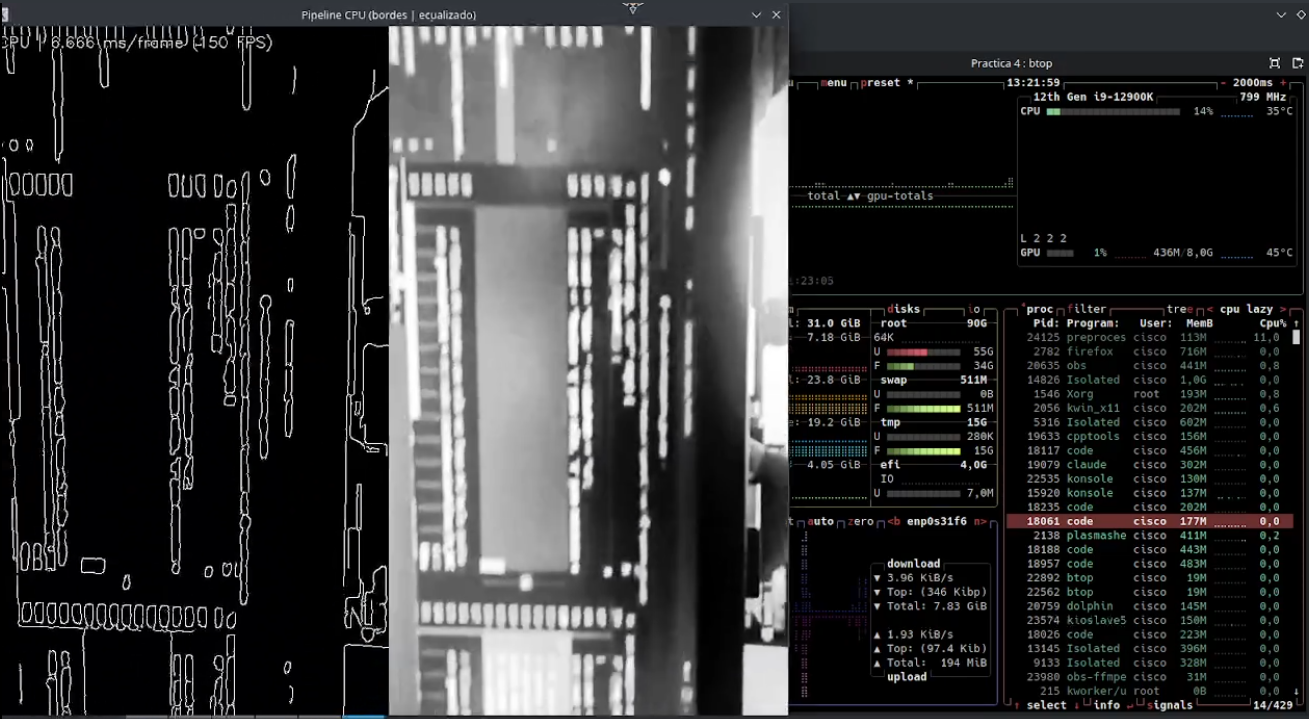
\includegraphics[width=0.95\textwidth]{imagenes/sectionC/bordes_cpu1.png}
  \caption{Pipeline CPU (bordes\,$|$\,ecualizado): 6.666\,ms/cuadro (150 FPS);
           \texttt{btop} registra 14\,\% de CPU y GPU ociosa (1\,\%).}
  \label{fig:bordes_cpu}
\end{figure}

\begin{figure}[H]
  \centering
  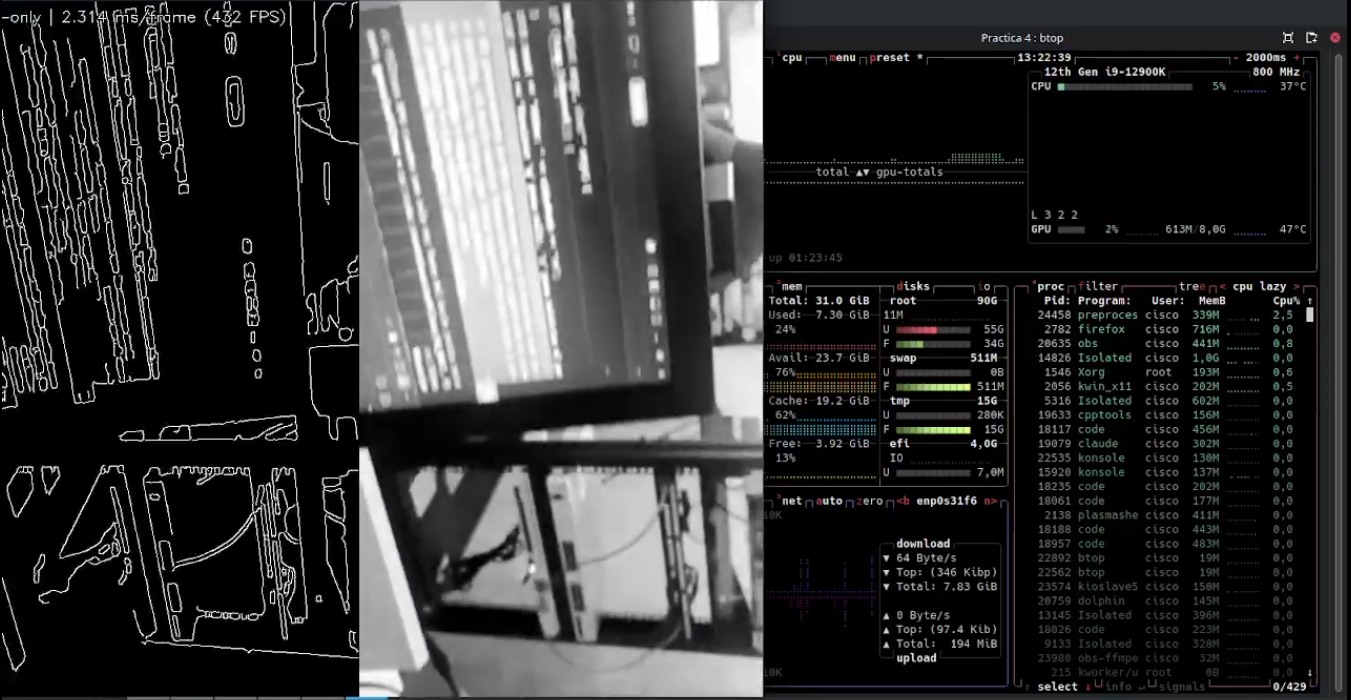
\includegraphics[width=0.95\textwidth]{imagenes/sectionC/bordes_gpu1.png}
  \caption{Pipeline GPU-only: 2.314\,ms/cuadro (432 FPS); el uso de CPU cae a
           5\,\% y la VRAM sube a 613\,MiB totales del sistema.}
  \label{fig:bordes_gpu}
\end{figure}

\begin{figure}[H]
  \centering
  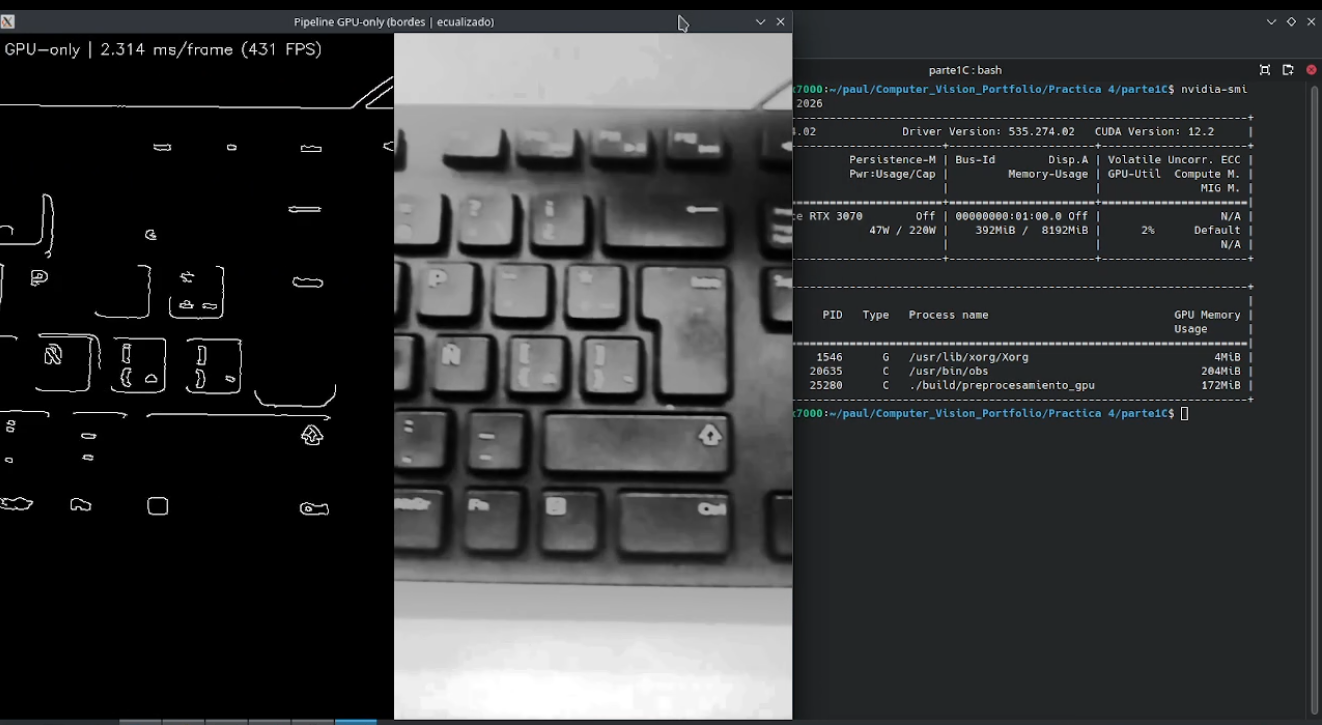
\includegraphics[width=0.95\textwidth]{imagenes/sectionC/gpu_nvidia_smi.png}
  \caption{\texttt{nvidia-smi} durante la corrida GPU del caso C: RTX 3070 al
           2\,\% de utilización, 47\,W/220\,W, con el proceso
           \texttt{preprocesamiento\_gpu} ocupando 172\,MiB de VRAM.}
  \label{fig:nvidia_smi_c}
\end{figure}

\subsection{Cuadro Comparativo Global y Discusión}

\begin{table}[H]
\centering
\caption{Resumen comparativo CPU vs.\ GPU de los tres casos de prueba.}
\label{tab:global}
\setlength{\tabcolsep}{4.5pt}
\small
\begin{tabular}{llccc}
  \toprule
  \textbf{Caso} & \textbf{Carga} & \textbf{CPU} & \textbf{GPU} & \textbf{Speedup} \\
  \midrule
  A & Entrenamiento YOLO26n-seg (60 ép.) & 3.5--4\,h & $\approx$90\,min & 2.4--2.7$\times$ \\
  A & Inferencia local (imagen)          & 98.6\,ms  & ---              & --- \\
  B & YOLOv12n video                     & 29.3 FPS  & 122.4 FPS        & 4.2$\times$ \\
  B & YOLO26n video                      & 38.9 FPS  & 124.8 FPS        & 3.2$\times$ \\
  B & Real-ESRGAN (cuadro completo)      & 4.40\,s   & 1.12\,s          & 3.9$\times$ \\
  B & Real-ESRGAN (recorte en vivo)      & 0.36 FPS  & 1.57 FPS         & 4.4$\times$ \\
  C & Bordes C++ OpenCV                  & 6.67\,ms (150 FPS) & 2.31\,ms (432 FPS) & 2.9$\times$ \\
  \bottomrule
\end{tabular}
\end{table}

\begin{table}[H]
\centering
\caption{Consumo de recursos observado durante las pruebas.}
\label{tab:recursos}
\setlength{\tabcolsep}{4.5pt}
\small
\begin{tabular}{llll}
  \toprule
  \textbf{Prueba} & \textbf{CPU (\%) / temp.} & \textbf{RAM} & \textbf{VRAM} \\
  \midrule
  A entren.\ GPU (T4)      & pipeline de datos       & 6.3\,GiB usados & 3.31--4.6\,GiB \\
  A entren.\ CPU (Xeon)    & 87--100\,\% / ---       & 5.2\,GiB proc.\ & --- \\
  B YOLO modo CPU          & núcleos 27--84\,\% / 67--70\,$^{\circ}$C & 7.5\,GiB & 436\,MiB (base) \\
  B YOLO modo CUDA         & 6--7\,\% / 51\,$^{\circ}$C  & 7.65\,GiB & 743\,MiB \\
  B ESRGAN modo CPU        & 52\,\% agreg.\ / 91\,$^{\circ}$C & 7.39\,GiB & 436\,MiB (base) \\
  B ESRGAN modo CUDA       & 5\,\% / 44\,$^{\circ}$C     & 7.44\,GiB & 899\,MiB \\
  C bordes modo CPU        & 14\,\% / 35\,$^{\circ}$C    & 7.18\,GiB & 436\,MiB (base) \\
  C bordes modo GPU        & 5\,\% / 37\,$^{\circ}$C     & 7.30\,GiB & 613\,MiB (172 del proceso) \\
  \bottomrule
\end{tabular}
\end{table}

\paragraph{¿Por qué gana la GPU en cada caso, y por cuánto?}
Los tres casos ilustran regímenes distintos de la misma ley: el speedup depende
de la razón entre cómputo paralelizable y costo de transferencia.

\begin{itemize}
  \item \textbf{Caso A (entrenamiento).} El entrenamiento es el escenario más
        favorable a la GPU: convoluciones y retropropagación son
        multiplicaciones matriciales masivas que saturan los SM, y el dataset
        reside en VRAM por lotes. El speedup observado (2.4--2.7$\times$)
        está acotado por la modestia de la T4 y por el pipeline de datos
        (decodificación JPEG y aumentos corren en una CPU de solo 2 vCPU); con
        una CPU anfitriona más capaz el margen crecería.
  \item \textbf{Caso B (inferencia profunda).} En redes convolucionales de
        inferencia el cómputo por cuadro sigue dominando sobre la
        transferencia de un único cuadro, de ahí los 3.2--4.4$\times$. El
        techo común de $\approx$125 FPS de ambas YOLO en GPU demuestra el
        efecto Amdahl: acelerada la red, mandan las etapas secuenciales de CPU
        (decodificación y dibujo). Real-ESRGAN, con 23 bloques residuales
        sobre cada píxel, es directamente inviable en CPU para uso interactivo
        (0.36 FPS y 91\,$^{\circ}$C sostenidos).
  \item \textbf{Caso C (procesamiento clásico).} Filtros gaussianos,
        morfología y Canny son operaciones de baja intensidad aritmética
        (memoria-limitadas). Aun así la GPU logra 2.9$\times$ porque el
        pipeline mantiene los datos en VRAM entre etapas (una sola subida y
        una sola bajada por cuadro); si cada operación viajara por PCIe, la
        latencia de transferencia anularía la ganancia. La utilización del
        2\,\% en \texttt{nvidia-smi} confirma que los kernels terminan casi
        instantáneamente y el tiempo restante es transferencia y
        sincronización: la GPU está sobredimensionada para esta carga.
\end{itemize}

\paragraph{Recomendaciones de uso.}
(i)~Entrenar y afinar redes profundas siempre en GPU; la CPU solo es admisible
para pruebas de humo. (ii)~Para inferencia en video con modelos nano, una CPU
de gama alta alcanza tiempo real ($\approx$30--39 FPS), por lo que la GPU se
justifica cuando se requieren múltiples flujos, modelos mayores o menor consumo
energético y térmico. (iii)~Para superresolución u otras redes generativas, la
GPU es obligatoria en cualquier escenario práctico. (iv)~En preprocesamiento
clásico, migrar a CUDA solo si el pipeline encadena varias etapas en VRAM y la
resolución o el número de flujos lo exige; a $480$p una CPU moderna ya excede
el tiempo real con amplio margen.

% ============================================================
\section{Conclusiones}
% ============================================================

La evidencia recogida en los tres benchmarks permite concluir lo siguiente:

\begin{enumerate}
  \item La GPU aceleró todas las cargas evaluadas, pero con magnitudes muy
        distintas según la naturaleza del cómputo: 2.4--2.7$\times$ en el
        entrenamiento de YOLO26n-seg (limitado por la T4 y el pipeline de
        datos de 2 vCPU), 3.2--4.4$\times$ en inferencia profunda sobre video
        (YOLO y Real-ESRGAN en la RTX 3070) y 2.9$\times$ en el pipeline
        clásico de bordes en C++. El factor determinante es la razón entre
        cómputo paralelizable y latencia de transferencia CPU$\leftrightarrow$VRAM.
  \item El fine-tuning convergió correctamente: la pérdida de clasificación
        cayó de 4.503 a 0.401 entre las épocas 1 y 60 y el mAP50 de cajas
        subió de 0.192 a 0.792, con un consumo estable de VRAM de
        3.31--4.6\,GiB, muy por debajo de los 15\,GiB de la T4.
  \item En inferencia GPU ambas variantes YOLO convergieron a
        $\approx$122--125 FPS pese a rendir distinto en CPU (29.3 vs.\ 38.9
        FPS), lo que demuestra que, una vez acelerada la red, el cuello de
        botella se traslada a las etapas secuenciales del bucle (decodificación
        y visualización), en concordancia con la ley de Amdahl.
  \item El costo sistémico de forzar cargas profundas en CPU es severo:
        Real-ESRGAN llevó al i9-12900K a 91\,$^{\circ}$C con 52\,\% de uso
        agregado para entregar 0.36 FPS, mientras la GPU resolvió la misma
        carga a 1.57 FPS con la CPU al 5\,\%. La GPU no solo es más rápida:
        libera al resto del sistema.
  \item En procesamiento clásico, la CPU ya supera el tiempo real (150 FPS a
        480p), por lo que la aceleración CUDA (432 FPS, 2\,\% de utilización,
        172\,MiB de VRAM) solo se justifica en resoluciones mayores, múltiples
        flujos o pipelines más profundos; el diseño de una única subida y una
        única bajada por cuadro fue la condición necesaria para que la GPU
        ganara en este caso.
\end{enumerate}

% ============================================================
\section*{Referencias}
\addcontentsline{toc}{section}{Referencias}
% ============================================================

\begin{thebibliography}{9}

\bibitem{Owens2008}
J.~D. Owens, M.~Houston, D.~Luebke, S.~Green, J.~E. Stone y J.~C. Phillips,
``GPU Computing,'' \textit{Proceedings of the IEEE}, vol.~96, n.º~5,
pp.~879--899, 2008.
\url{https://doi.org/10.1109/JPROC.2008.917757}

\bibitem{NVIDIA_CUDA}
NVIDIA Corporation, \textit{CUDA C++ Programming Guide}, versión 12.x, 2025.
\url{https://docs.nvidia.com/cuda/cuda-c-programming-guide/}

\bibitem{Paszke2019}
A.~Paszke \textit{et al.}, ``PyTorch: An Imperative Style, High-Performance
Deep Learning Library,'' en \textit{Advances in Neural Information Processing
Systems 32 (NeurIPS)}, 2019.
\url{https://arxiv.org/abs/1912.01703}

\bibitem{Ultralytics}
Ultralytics, \textit{Ultralytics YOLO Documentation}, 2026.
\url{https://docs.ultralytics.com/}

\bibitem{Wang2021}
X.~Wang, L.~Xie, C.~Dong y Y.~Shan, ``Real-ESRGAN: Training Real-World Blind
Super-Resolution with Pure Synthetic Data,'' en \textit{IEEE/CVF International
Conference on Computer Vision Workshops (ICCVW)}, 2021, pp.~1905--1914.
\url{https://doi.org/10.1109/ICCVW54120.2021.00217}

\bibitem{OpenCV_CUDA}
OpenCV, \textit{CUDA Module Introduction --- GPU-Accelerated Computer Vision},
documentación oficial.
\url{https://docs.opencv.org/4.x/d2/dbc/cuda_intro.html}

\bibitem{Canny1986}
J.~Canny, ``A Computational Approach to Edge Detection,'' \textit{IEEE
Transactions on Pattern Analysis and Machine Intelligence}, vol.~PAMI-8,
n.º~6, pp.~679--698, 1986.
\url{https://doi.org/10.1109/TPAMI.1986.4767851}

\end{thebibliography}

% ============================================================
\appendix
\section{Anexos}
% ============================================================

\subsection{Repositorio y Material Complementario}

Los videos de demostración de las tres partes de la práctica se encuentran
disponibles en la siguiente carpeta de Google Drive:

\begin{center}
  \url{https://drive.google.com/drive/folders/1QBBWjK9oUn1fayTIRIUvuzareJY8L_fN?usp=sharing}
\end{center}

El código fuente completo (cuadernos de Colab, scripts de la Parte 1B y
proyecto C++ de la Parte 1C) se encuentra disponible en:

\begin{center}
  % TODO: reemplazar cuando se suba el repositorio
  \texttt{[ENLACE AL REPOSITORIO -- pendiente]}
\end{center}

\subsection{Estructura del Proyecto}

\begin{lstlisting}[style=code]
Practica 4/
|-- parte1A/                 # Caso A: fine-tuning YOLO26n-seg
|   |-- 01_Practica4_YOLO26_Segmentacion.ipynb
|   |-- 02_Practica4_Inferencia_Local.ipynb
|   |-- 03_Practica4_Benchmark_Hardware_Colab.ipynb
|   `-- save/                # metricas, capturas y demos generadas
|-- parte1B/                 # Caso B: inferencia YOLO y Real-ESRGAN
|   |-- run_yolo.py
|   |-- run_superres.py
|   `-- modelos/             # yolo12n.pt, yolo26n.pt, RealESRGAN_x4plus.pth
`-- parte1C/                 # Caso C: pipeline C++ OpenCV/CUDA
    |-- CMakeLists.txt
    |-- Makefile
    `-- src/
        |-- pipeline_cpu.cpp
        `-- pipeline_gpu.cpp
\end{lstlisting}


\end{document}
